\subsection{Análise da aplicação de revestimento}

Atualmente, as mangueiras que conduzem o gás de arraste do pó até o
reservatório (hooper) possui 5m. Nas condições de aplicação de revestimento
\textit{in situ}, o posicionamento do reservatório dentro da turbina pode chegar
a 25m do painel alimentador, logo os comprimentos das mangueiras foram trocas
para simular a aplicação. O objetivo foi avaliar a qualidade do revestimento
aplicado nas condições \textit{in situ}, e o equipamento Accura Spray através
da produção de corpos de prova. Os testes de qualificação do revestimento são:
dobramento, dureza, adesão e metalografia.

As atividades tiveram o intuito de simular a perda de carga dos gases
combustíveis e de arraste da partícula quando \textit{in situ}. As etapas
realizadas foram: substituição das mangueiras que conduzem o gás de arraste (N2)
até o reservatório de pó; substituição das mangueiras de propano e oxigênio;
substituição das mangueiras de água de refrigeração da pistola de coating;
acionamento da pistola, movimentação do manipulador e monitoramento com o sensor
de chama (Accura Spray).

Os resultados estão apresentados na Tabela~\ref{tab:hvof_tab2}. Os parâmetros
utilizados durante a execução dos testes estão na Tabela~\ref{tab:hvof_tab3}. Os
mesmos parâmetros foram utilizados para os testes de altura. Outros três testes
foram realizados a partir das condições apresentadas na
Tabela~\ref{tab:hvof_tab2}. As modificações nos parâmetros no console foram
monitoradas pelo sensor de chama Accura Spray. Os resultados observados estão
resumidos na Tabela~\ref{tab:hvof_tab4}.

\begin{table}[]
\centering
\caption{Resultados dos teste de metalização em longas distâncias}
\label{tab:hvof_tab2}
\begin{tabular}{|c|l|}
\hline
\begin{tabular}[c]{@{}c@{}}Estabilização\\ da chama\end{tabular} & \begin{tabular}[c]{@{}l@{}}Etapa inicial foi normal em termos \\ de tempo e fluxo de material, condizente\\ com o utilizado atualmente.\end{tabular}                                                                                                                        \\ \hline
\begin{tabular}[c]{@{}c@{}}Teste\\ dinâmico\end{tabular}         & \begin{tabular}[c]{@{}l@{}}Não houve variação visual da chama \\ durante movimentação do robô nos\\ sentidos vertical e horizontal.\end{tabular}                                                                                                                            \\ \hline
\begin{tabular}[c]{@{}c@{}}Teste\\ estático\end{tabular}         & \begin{tabular}[c]{@{}l@{}}O teste de monitoramento com o sensor\\ mostrou uma variação de velocidade da \\ chama dentro dos limites aceitáveis para \\ esse critério: de 550 a 750 m/s. A \\ observação foi realizada durante 30 min \\ com a pistola ligada.\end{tabular} \\ \hline
\end{tabular}
\end{table}

\begin{table}[]
\centering
\caption{Parâmetros}
\label{tab:hvof_tab3}
\begin{tabular}{|c|l|}
\hline
\begin{tabular}[c]{@{}c@{}}Propano\\ Vazão/Pressão\end{tabular}  & 35 FMR/100 Psi \\ \hline
\begin{tabular}[c]{@{}c@{}}Oxigênio\\ Vazão/ Presão\end{tabular} & 35 FMR/150 Psi \\ \hline
Ar comprimido Vazão/Presão                                       & 42 FMR/100 Psi \\ \hline
\end{tabular}
\end{table}

\begin{table}[]
\centering
\caption{Resultados observados durante teste de modificação de parâmetros no
console de vazão de gases e distância de aspersão.}
\label{tab:hvof_tab4}
\begin{tabular}{ll}
\hline
Modificação                                                                                                             & Resultado observado                                                                                                                                                                                                                                                                                      \\ \hline
\multicolumn{1}{|l|}{\begin{tabular}[c]{@{}l@{}}Variação na taxa de aspersão: \\ 40g/min para 15g/min\end{tabular}}     & \multicolumn{1}{l|}{Foi aumentada a velocidade da chama.}                                                                                                                                                                                                                                                \\ \hline
\multicolumn{1}{|l|}{\begin{tabular}[c]{@{}l@{}}Variação na vazão de Ar no console:\\ 45scfh para 30 scfh\end{tabular}} & \multicolumn{1}{l|}{\begin{tabular}[c]{@{}l@{}}Tanto o aumento como a diminuição \\ da vazão de ar provocaram a diminuição \\ da velocidade da chama, ficando evidente \\ que existe um ponto ótimo que deve ser \\ ajustado de acordo com a condição da\\ instalação de todo equipamento.\end{tabular}} \\ \hline
\multicolumn{1}{|l|}{\begin{tabular}[c]{@{}l@{}}Variação da distância de aspersão:\\ 230 mm para 50 mm\end{tabular}}    & \multicolumn{1}{l|}{\begin{tabular}[c]{@{}l@{}}A velocidade da chama variou de\\ aproximadamente 700 m/s para 1056 m/s.\\ Enquanto que a temperatura subiu de \\ 1600°C para 1700°C aprox.\end{tabular}}                                                                                                 \\ \hline
\end{tabular}
\end{table}


Após a modificação descrita acima, o comprimento da mangueira de água foi
subs\-tituído por 30m, e a instalação de uma bomba hidráulica para a aplicação
em 0 m até 4 m. A substituição das mangueiras do gás de arraste desde o console do alimentador até o reservatório de pó consiste na retirada das mangueiras em
todas as conexões que vão do reservatório até o console, instalação das
mangueiras novas, e avaliação do funcionamento da máquina nessa nova condição.
Da mesma forma, o objetivo foi avaliar o funcionamento do equipamento através do uso do Accura Spray.

A aplicação em altura foi realizada da seguinte forma: 
após substituição das man\-guei\-ras, a pistola de revestimento foi posicionada
no nível de zero metros; o sensor de chama foi posicionado perpendicularmente à
pistola de coating e a uma distância de 230mm; a pistola foi acionada (ignição) e
os ajustes de vazão dos gases foram realizados; o alimentador de pó foi
acionado para inicialização do fluxo de pó e os ajustes da vazão foram
realizados. 

A etapa inicial de queima é a estabilização da chama, onde a variação de vazão
de pó no console e o aspecto da chama é observado antes do início da aspersão
propriamente (ou seja, antes da aplicação do pó na peça ou amostra). Após a
estabilização, a aspersão foi observada pelo sensor de chama Accura Spray e o
valor foi registrado. Após o registro da temperatura e velocidade da chama, os
corpos de prova foram metalizados. Repetiu-se esse procedimento para as alturas
de 1.3; 2.6 e 4 m.

O cabeçote do equipamento Accura Spray é montado em um tripé, perpendicular e
distante 8 polegadas da linha da chama de aspersão e a 230 mm de distância
(essa distância varia conforme o intuito do teste ou conforme o pó utilizado)
do bocal da pistola de aspersão. O Accura Spray é operado por meio de software
específico. A Fig.~\ref{fig:adequacao1} apresenta o notebook contendo o
programa para operação do equipamento fora da cabine com o cabeçote (ao fundo)
no interior da cabine.

\begin{figure}
	\centering
	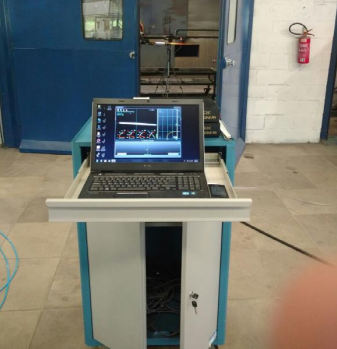
\includegraphics[width=1\columnwidth]{method/figs/adequacao/adequacao1.png}
    \caption{Monitoramento da temperatura e velocidade da chama de aspersão
    (janeiro de 2016).}
    \label{fig:adequacao1}
\end{figure}

As vazões e pressões dos gases de combustão do processo durante o teste de
operação da pistola em longas distâncias é regulado no console do equipamento
enquanto que o resultado da medição dos parâmetros de chama durante o teste é
visualizado no notebook com o software do Accura Spray.

A montagem e realização dos testes de operação com variação da altura de
aspersão são realizadas juntamente com o ajuste do equipamento Accura Spray na
condição de operação mais baixa possível, próximo a 0 m. Após o posicionamento
do robô e do accura spray é realizado a avaliação inicial da chama para a
altura de 0 m. Da mesma forma anterior, os parâmetros de chama medidos nessas
condições são visualizados na interface do accura spray.

Para a execução dos testes utilizando o manipulador com a pistola em posições
mais elevadas foi realizada a instalação de uma bomba para evitar a queda da
pressão de água de refrigeração da pistola. Após o posicionamento, teve de ser
realizada uma aferição visual do paralelismo do cabeçote com a chama de
aspersão, para evitar desvios na medição. Na ultima etapa desse teste foi
realizada aspersão com o manipular posicionado em 4 m de altura, juntamente com
instalação do cabeçote do Accura Spray conforme Fig.~\ref{fig:adequacao2}.

A Tabela~\ref{tab:hvof_tab5} apresenta os resultados registrados pelo sensor de
chama.

\begin{table}[]
\centering
\caption{Valores registrados pelo sensor de chama Accura spray no teste de
metalização em diferentes alturas do braço robótico.}
\label{tab:hvof_tab5}
\begin{tabular}{lll}
\hline
\begin{tabular}[c]{@{}l@{}}Altura\\ de aspersão (m)\end{tabular} & \begin{tabular}[c]{@{}l@{}}Velocidade\\ da chama (m/s)\end{tabular} & \begin{tabular}[c]{@{}l@{}}Temperatura\\ da chama (°C)\end{tabular} \\ \hline
\multicolumn{1}{|l|}{0}                                          & \multicolumn{1}{l|}{608}                                            & \multicolumn{1}{l|}{1592}                                           \\ \hline
\multicolumn{1}{|l|}{1.3}                                        & \multicolumn{1}{l|}{682}                                            & \multicolumn{1}{l|}{1553}                                           \\ \hline
\multicolumn{1}{|l|}{2.6}                                        & \multicolumn{1}{l|}{630}                                            & \multicolumn{1}{l|}{1632}                                           \\ \hline
\multicolumn{1}{|l|}{4}                                          & \multicolumn{1}{l|}{588}                                            & \multicolumn{1}{l|}{1590}                                           \\ \hline
\end{tabular}
\end{table}

\begin{figure}
	\centering
	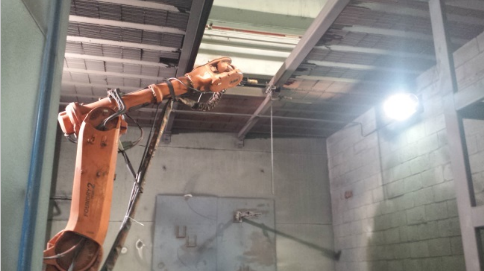
\includegraphics[width=1\columnwidth]{method/figs/adequacao/adequacao2.png}
    \caption{Posicionamento do robô e programação do movimentador,
    posicionamento dos corpos de prova e do Accura Spray para aplicação em 4 
    metros (janeiro de 2016).}
    \label{fig:adequacao2}
\end{figure}
